\section{Introduction}

    % Interference double-silt source: https://wiki.anton-paar.com/ch-de/doppelspaltexperiment/
    % Interference grating source: https://www.grund-wissen.de/physik/optik/wellenoptik.html
    % Grating constant source: https://ieeexplore.ieee.org/stamp/stamp.jsp?tp=&arnumber=5547333&tag=1 (eth network)
    % Lands Pits CD source: https://www.researchgate.net/figure/Lands-and-pits-image-using-a-scanning-electron-microscope_fig3_221291847
    

    The goal of this experiment series is to build a spectrometer using household objects by making use of the wave character of light.
    To understand how the spectrometer works, we need to take a close look at how light behaves under certain conditions.

    \begin{figure}[H]
        \centering
        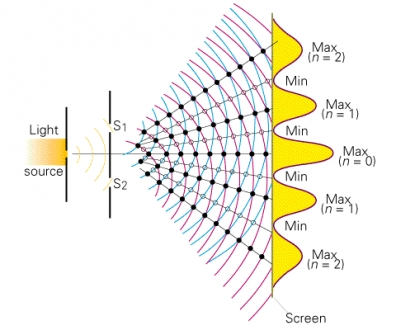
\includegraphics[scale = 0.7]{src/images/interference_double_slit.jpg}
        \caption{Double slit experiment.
        The interference of the light waves produce aspecific pattern which depends of the wavelength of the light entering the slits as well as the distance between the slits. \cite{src_double_slit}}
        \label{fig_double_slit}
    \end{figure}

    Light travels in a spherical way behind a slit meaning that each slit acts as a new source of waves.
    These waves interfere with each other as they overlap, resulting in an interference pattern of alternating bright and dark regions on the screen or detector.
    This behaviour is due to the fact that two maxima or minima intensify each other while a maximum and a minimum cancel out.
    We also refer to these two cases as constructive and destructive.
    Figure~\ref{fig_double_slit} shows how this effect works.

    \begin{minipage}{0.99\linewidth}
        \begin{minipage}{0.7\linewidth}
            \begin{figure}[H]
                \centering
                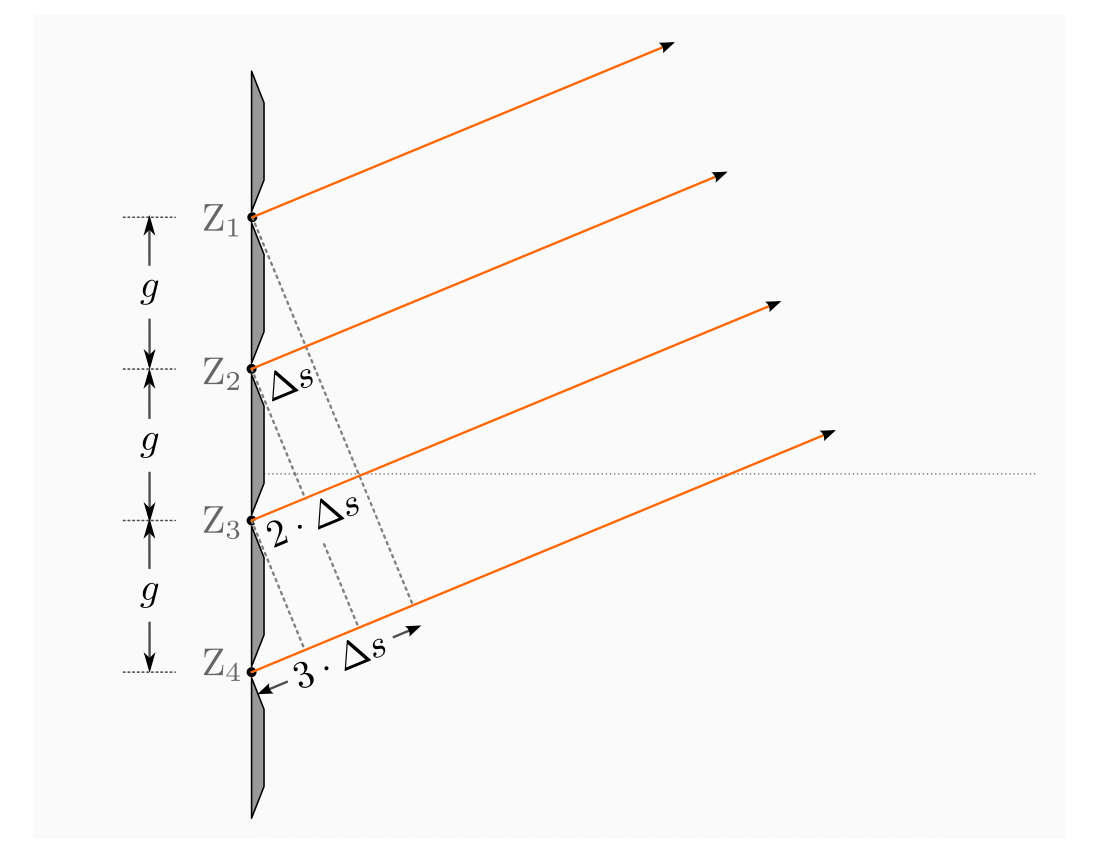
\includegraphics[scale = 0.25]{src/images/interference_grating.png}
                \caption{A grating leads to a similar effect as a double slit.
                $\Delta s$ is equal to the wavelength.
                As seen in the figure, the angle at which brighter spots of light can be seen depends on the wavelength. \cite{src_grating}}
                \label{fig_grating}
            \end{figure}
        \end{minipage}
        \begin{minipage}{0.25\linewidth}
          \begin{scriptsize}
            \begin{center}
                \begin{figure}[H]
                    \centering
                    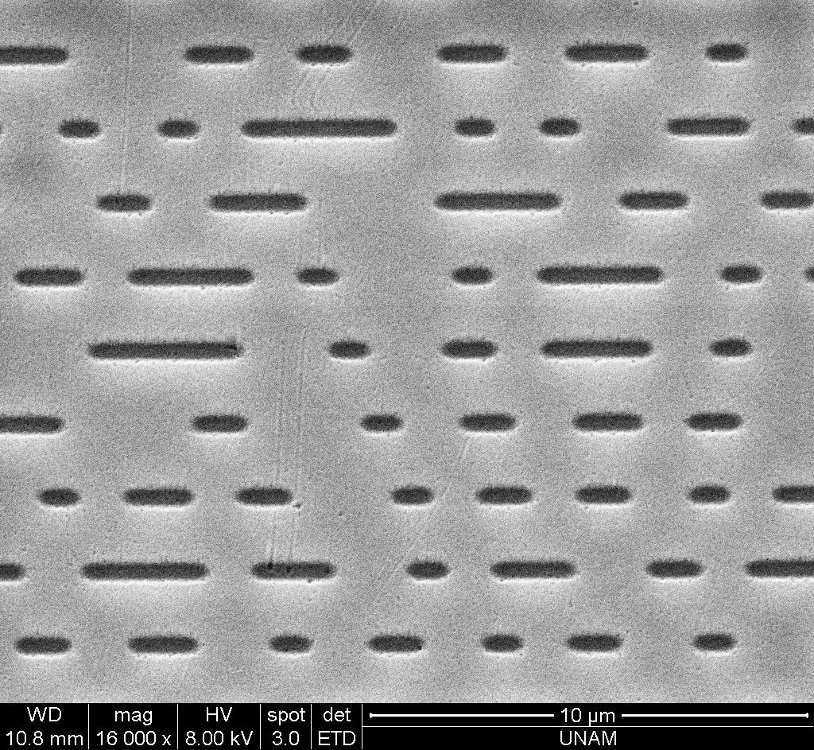
\includegraphics[scale = 0.15]{src/images/lands_pits_cd.png}
                    \caption{Lands and pits image of a CD using a scanning electron microscope. These form a grating too. \cite{src_cd}}
                    \label{fig_lands_pits}
                \end{figure}
            \end{center}
            \end{scriptsize}
        \end{minipage}
    \end{minipage}

    Moving on to a grating, it can be abstracted as a lot of slits next to each other.
    Hence, the effect is almost the same as the one observed at the double slit.
    Most importantly, an interference pattern can be observed too.
    When taking a close look at a CD, we notice a grating, presented in figure~\ref{fig_lands_pits}.
    In consequence, a CD must also produce an interference pattern in which light of different wavelength can be observed and distinguished.
    The characterisation of the light is done by measuring the distance between the maximum of first and zero order as it is dependent of the wavelength.

    \begin{minipage}{0.99\linewidth}
        \begin{minipage}{0.45\linewidth}
            \begin{figure}[H]
                \centering
                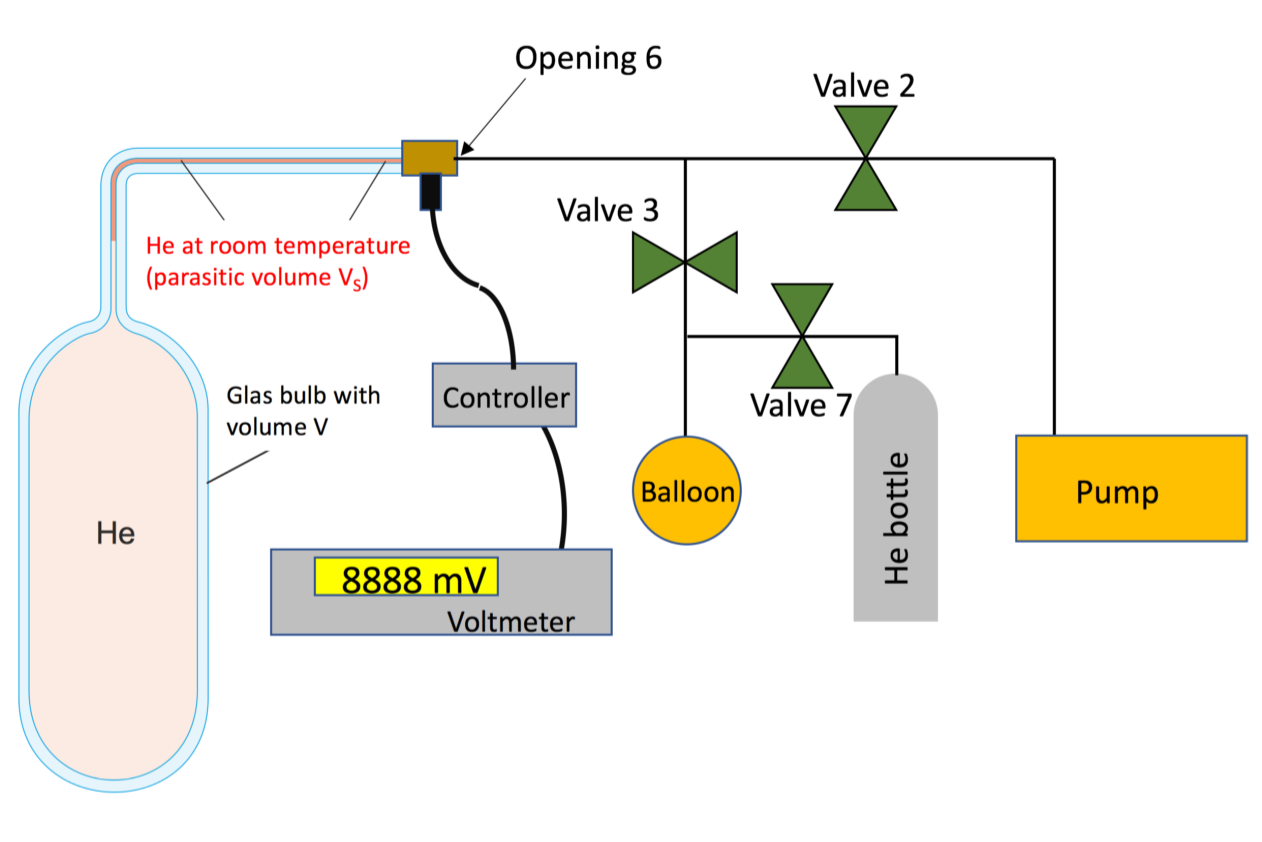
\includegraphics[scale = 0.4]{src/images/experimental_setup.png}
                \caption{Schematic of the experimental setup.
                A source emits rays of light of which a small portion enters the apparatus through a gap between two razor blades of about 0.2 mm.
                the light then travels through the dark chamber, until it hits the CD.
                After passing through the grid on the CD, an interference pattern can be detected using a camera.}
                \label{fig_setup}
            \end{figure}
        \end{minipage}
        \begin{minipage}{0.1\linewidth}
        \end{minipage}
        \begin{minipage}{0.45\linewidth}
          \begin{scriptsize}
            \begin{center}
                \begin{figure}[H]
                    \centering
                    \includegraphics[scale = 0.05]{src/images/spectrometer.png}
                    \caption{Experimental setup used in our case.
                    A phone is used as the camera to detect the interference pattern.}
                    \label{fig_spectrometer}
                \end{figure}
            \end{center}
            \end{scriptsize}
        \end{minipage}
      \end{minipage}
    


    % In general this section should tell the reader why he or she should
    % be interested in your paper. Give some background to the
    % experiment, and describe the underlying principles. This is typically where you provide references to previous publications~\cite{Sato2003}.